%-----------------------------------------
% To process this file:
%   pdflatex fpp-manual
%   bibtex fpp-manual
%   pdflatex fpp-manual
%   pdflatex fpp-manual
%-----------------------------------------

%\documentclass{article}
\documentclass{hitec}     % Tutorial overall style

\usepackage{index}
\usepackage{xr}
\usepackage{textgreek}
\usepackage{setspace}
\usepackage{graphicx}
\usepackage{moreverb}    % Defines {listing} environment.
\usepackage{amsmath, amsthm, amssymb, amsbsy, mathtools}
\usepackage{alltt}
\usepackage{rotating}
\usepackage{enumitem}
\usepackage{subcaption}
\usepackage{toc-dcs}    % See toc-dcs.sty file in this directory.
\usepackage{xspace}
%%\usepackage{makeidx}
\usepackage[section]{placeins}   % For preventing floats from floating to end of chapter.
\usepackage{longtable}  % For splitting long vertical tables into pieces
\usepackage{multirow}
\usepackage{booktabs}   % For table layouts
\usepackage{yhmath}     % For widehat
\usepackage{mathpazo}   % Make math equations look a bit bolder.
\usepackage{xcolor}     % Needed for listings package.
\usepackage{listings}
\usepackage[T1]{fontenc}   % so _, <, and > print correctly in text.
\usepackage[strings]{underscore}    % to use "_" in text
\usepackage[nottoc,numbib]{tocbibind}   % Makes "References" section show in table of contents
\usepackage[pdftex,colorlinks=true,bookmarksnumbered=true]{hyperref}   % Must be last package!

%----------------------------------------------------------------

\newcommand{\extref}[1]{$\S$\ref*{#1}}   % No hyperlink. For external refs. \extref
\newcommand{\comma}{\> ,}
\newcommand{\period}{\> .}
\newcommand{\wt}{\widetilde}
\newcommand{\grv}{\textasciigrave}
\newcommand{\hyperbf}[1]{\textbf{\hyperpage{#1}}}
\newcommand{\Ss}{\(^*\)}
\newcommand{\Dd}{\(^\dagger\)}

\newcommand{\AND}{&& \hskip -17pt\relax}
\newcommand{\CR}{\\}
\newcommand{\CRNO}{\nonumber \\}
\newcommand{\dstyle}{\displaystyle}

\newcommand{\Begineq}{\begin{equation}}
\newcommand{\Endeq}{\end{equation}}
\newcommand{\NoPrint}[1]{}

\newcommand{\pow}[1]{\cdot 10^{#1}}
\newcommand{\Bf}[1]{{\bf #1}}
\newcommand{\bfr}{\Bf r}

\newcommand{\bmad}{{\sl Bmad}\xspace}
\newcommand{\tao}{{\sl Tao}\xspace}
\newcommand{\mad}{{\sl MAD}\xspace}
\newcommand{\cesr}{{\sl CESR}\xspace}

\newcommand{\sref}[1]{\S\ref{#1}}
\newcommand{\Sref}[1]{Sec.~\sref{#1}}
\newcommand{\cref}[1]{Chapter~\ref{#1}}

\newcommand{\Newline}{\hfil \\ \relax}

\newcommand{\eq}[1]{{(\protect\ref{#1})}}
\newcommand{\Eq}[1]{{Eq.~(\protect\ref{#1})}}
\newcommand{\Eqs}[1]{{Eqs.~(\protect\ref{#1})}}

\newcommand{\vn}{\ttcmd}           % For variable names
\newcommand{\vni}{\ttcmdindx}
\newcommand{\cs}{\ttcmd}           % For code source
\newcommand{\cmd}{\ttcmd}          % For Unix commands
\newcommand{\rn}{\ttcmd}           % For Routine names
\newcommand{\tn}{\ttcmd}           % For Type (structure) names
\newcommand{\bn}[1]{{\bf #1}}       
\newcommand{\toffset}{\vskip 0.01in}
\newcommand{\rot}[1]{\begin{rotate}{-45}#1\end{rotate}}

\newcommand{\data}{{\mbox{data}}}
\newcommand{\reference}{{\mbox{ref}}}
\newcommand{\model}{{\mbox{model}}}
\newcommand{\base}{{\mbox{base}}}
\newcommand{\design}{{\mbox{design}}}
\newcommand{\meas}{{\mbox{meas}}}
\newcommand{\var}{{\mbox{var}}}

\newcommand\ttcmd{\begingroup\catcode`\_=11 \catcode`\%=11 \dottcmd}
\newcommand\dottcmd[1]{\texttt{#1}\endgroup}

\newcommand\ttcmdindx{\begingroup\catcode`\_=11 \catcode`\%=11 \dottcmdindx}
\newcommand\dottcmdindx[1]{\texttt{#1}\endgroup\index{#1}}

\newcommand{\St}{$^{st}$\xspace}
\newcommand{\Nd}{$^{nd}$\xspace}
\newcommand{\Th}{$^{th}$\xspace}
\newcommand{\B}{$\backslash$}
\newcommand{\W}{$^\wedge$}

\newcommand{\cbar}[1]{\overline C_{#1}}

\newlength{\dPar}
\setlength{\dPar}{1.5ex}

\newenvironment{example}
  {\vspace{-3.0ex} \begin{alltt}}
  {\end{alltt} \vspace{-2.5ex}}

\newcommand\Strut{\rule[-2ex]{0mm}{6ex}}

\newenvironment{Itemize}
  {\begin{list}{$\bullet$}
    {\addtolength{\topsep}{-1.5ex} 
     \addtolength{\itemsep}{-1ex}
    }
  }
  {\end{list} \vspace*{1ex}}

\newcommand{\Section}[1]{\section{#1}\indent\vspace{-3ex}}

\newcommand{\SECTION}[1]{\section*{#1}\indent\vspace{-3ex}}

% From pg 64 of The LaTex Companion.

\newenvironment{ventry}[1]
  {\begin{list}{}
    {\renewcommand{\makelabel}[1]{\textsf{##1}\hfil}
     \settowidth{\labelwidth}{\textsf{#1}}
     \addtolength{\itemsep}{-1.5ex}
     \addtolength{\topsep}{-1.0ex} 
     \setlength{\leftmargin}{5em}
    }
  }
  {\end{list}}


\definecolor{backcolor}{rgb}{0.8824,1.0,1.0}   % To match code environment
\lstset{basicstyle = \small, backgroundcolor=\color{backcolor}, escapeinside = {@!}{!@}}

\renewcommand{\textfraction}{0.1}
\renewcommand{\topfraction}{1.0}
\renewcommand{\bottomfraction}{1.0}

\settextfraction{0.9}  % Width of text
\setlength{\parindent}{0pt}
\setlength{\parskip}{1ex}
%\setlength{\textwidth}{6in}
\newcommand{\Section}[1]{\section{#1}\vspace*{-1ex}}

\newenvironment{display}
  {\vspace*{-1.5ex} \begin{alltt}}
  {\end{alltt} \vspace*{-1.0ex}}

\title{Fully Polymorphic Package Manual}
%\titlehead{adf}

\author{}
\date{
  \parbox{6in}{
\includegraphics[width=5in]{logo-fpp.pdf}\vspace*{0.4in}} \\ 
  Etienne Forest and David Sagan \\ 
  March 25, 2023
}

\begin{document}

\phantomsection
\pdfbookmark[1]{Cover Page}{Cover Page}
\maketitle

\cleardoublepage
\phantomsection
\pdfbookmark[1]{Contents}{Contents}
\tableofcontents

\newpage

%--------------------------------------------------------------------------------------------------------
\Section{Introduction to FPP/PTC}
\label{s:intro}

FPP/PTC is an object oriented, open source, subroutine library for
\begin{itemize}
\item The manipulation and analysis of Taylor series and Taylor maps.
\item Modeling of charged particle beams in accelerators using Taylor maps.
\end{itemize}
The popularity of FPP/PTC can be attested to by its use by the Bmad\cite{b:bmad} toolkit for
accelerator and X-ray simulations as well the MAD\cite{b:mad} simulation program.

FPP/PTC has two parts. The Fully Polymorphic Package (FPP) is the part that deals with Taylor series
and maps. FPP is pure math independent1 of any "physics". The Polymorphic Tracking Code (PTC) part
of the library deals with the modeling of particle beams and accelerators. PTC contains the
"physics" and relies on FPP for producing and manipulating Taylor maps.  This is illustrated in
Figure~\ref{f:ptc}. Roughly, FPP can be subdivided into two parts, a Taylor manipulation part for
basic manipulations of Taylor series and an analysis part to do things like normal form
analysis. PTC uses the Taylor manipulation part of FPP for things like the construction of Taylor
maps. Additionally, PTC uses the analysis tools of FPP. A closer look at FPP shows the existence of
a Differential Algebra (DA) package within FPP. This package was originally coded by Martin Berz.

This manual is focused on how to use FPP. Since FPP is designed to serve PTC there will be some
mention of PTC but only so far as how PTC relates to FPP. In particular, tracking through lattices
is not discussed and the reader is referred to the PTC documentation for this.

\begin{figure}[tb]
  \centering
  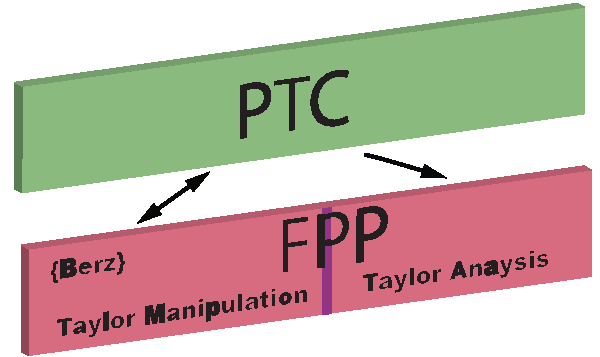
\includegraphics[width=0.8\textwidth]{ptc-fpp.pdf}
  \caption{
The Fully Polymorphic Package (FPP) part of the FPP/PTC library provides manipulation and analysis
of Taylor series and maps and the Polymorphic Tracking Code (PTC) part provides the physics from
which accelerators can be analyzed. Arrows indicate code dependencies. The Taylor analysis code uses
the Taylor manipulation code but not vice versa. FPP does not use PTC but PTC code uses both FPP's
Taylor manipulation and analysis.
  }
  \label{f:ptc}
\end{figure}

%--------------------------------------------------------------------------------------------------------
\Section{Where to Obtain FPP/PTC}
\label{s:obtain}

FPP/PTC can be downloaded from the web via the Bmad web site\cite{b:bmad} or at
\begin{code}
https://github.com/jceepf/fpp_book
\end{code}



%--------------------------------------------------------------------------------------------------------
\Section{Concepts}
\label{s:concepts}

%-------------------------------------------------------------------
\subsection{Conventions}
\label{s:conventions}

FPP/PTC is written in Fortran90. It is assumed that the reader has some familiarity with this
language. In particular, it is assumed that the reader knows what a \vn{structure} is (roughly
corresponding to a \vn{class} in Python or C++) which is also called a \vn{derived type}. Also it is
assumed that the reader knows about operator overloading.

FPP/PTC uses double precision numbers. The kind type parameter ``\vn{dp}'' is defined in FPP/PTC to
correspond to double precision numbers. For example:
\begin{code}
real(rp) abc, xyz             ! Declare double precision vars abc and xyz.
xyz = 3.4_dp * abc / 1e9_dp   ! 3.4_dp and 1e9_dp are double precision.
\end{code}

%-------------------------------------------------------------------
\subsection{TPSA Versus DA}
\label{s:tpsa}

TPSA stands for ``Truncated Power Series Algebra'' and DA stands for ``Differential Algebra.'' But
what does it mean when applied to a typical accelerator ring? Once we cut the mathematical jargon,
we will see that

\begin{itemize}
\item TPSA operations take into account the constant part and the results change as a function of the order. 
%
\item DA operations are equivalent to normal TPSA operations used around the closed orbit and thus the
constant part of the map is ignored. All the coefficients of the Taylor series stay the same
independently of the order invoked. It so happens that the computation of nonlinear differential
operators (Lie vector fields for example), are self-consistent because they form a differential
algebra. But it is much simpler in our field to state that they are self-consistent because there
are no feed down terms.
\end{itemize}

It is important to understand why a non-zero constant part of a Taylor series can be
problematical. To see this, consider TPSA maps of order $N$ from $x$ to $y$ and $y$ to $z$
\begin{align}
  y &= \sum_{j = 0}^N a_j x^j  \label{yj0n} \\
  z &= \sum_{j = 0}^N b_j y^j + \calO(y^{N+1}) \label{zj0n}
\end{align}
In \Eq{zjon} it is made explicit that are term of order $N+1$ or higher that are being negelted.
These maps can be concatenated to form a TPSA map of $z$ as a function of $x$ 
\begin{equation}
  z = \sum_{j = 0}^N c_j x^j
  \label{zj0n}
\end{equation}
If there is a neglected term in \Eq{zjon} that looks like $b_m y^m$ with $m > N$, substituting
\Eq{yjon} into this it is immediately seen that if, and only if, $a_0$ is non-zero, this neglected
term will (if it were not neglected) contribute to the coefficients $c_j$ in \Eq{zjon}. This is
called ``feed down''. That is, terms of higher order will affect the coefficients of lower order
terms when TPSA maps are combined. To avoid this, maps with zero constant term should be used. With
simulations, this generally means computing maps with respect to the nominal beam orbit. For
lattices with a closed geometry, this generally means computing maps with respect to the closed
orbit. For lattices with an open geometry (EG: Linacs), the reference orbit can be some orbit
defined by tracking a beam from some user-specified initial position.

%-------------------------------------------------------------------
\subsection{Polymorphism}
\label{s:poly}

In computer programming ``\vn{Polymorphism}'' is the property that a given variable, object, or
function can act in different ways depending upon the context. With FPP/PTC, polymorphism is used to
define types that can act as if the structure components were real valued numbers or Taylor series.
See the documentation of the \vn{real_8} type (\sref{s:real.8}) as an example.

The \vn{PTC} tracking code typically has two routines: with a ``p'' or ``r'' at the end...

Polymorphic types (\sref{s:poly}) generally (always???) have structure names that have a \vn{_8}
suffix.


ToDo: Give an example of a routine that uses real_8 or probe_8 as a scaler.

%-------------------------------------------------------------------
\subsection{Operator Overloading}
\label{s:overloading}

FPP/PTC heavily uses operator overloading for Taylor series manipulation. Not only are the standard
arithmetical operators ($+, -, *, /, **$) overloaded as well as the equal sign ($=$), but there are
a number of custom operators that are defined as well. Below is a list.\footnote
  {
Note: Fortran mandates that custom operator names begin and end with a dot ``.''.
  }
\begin{description}
\item[+, -] \Newline
Standard addition and subtraction of Taylor series.
%
\item[*] \Newline

%

\end{description}

%-------------------------------------------------------------------
\subsection{Tracking Versus Analysis}
\label{s:tracking.analysis}

An important distiction here is the difference between \vn{tracking} and \vn{analysis}. By
``tracking'' it is meant either the propagation through a lattice of a single particle or a
transport map (which here is always an array of truncated Taylor power series).\footnote
  {
Mathematically, single particle tracking is just tracking of a transport map using Taylor series
truncated at zeroth order. From the code perspective, due to the speed penelely with dealing with
Taylor series, the two are distinct as will be seen in this manual.
  }
This is opposed to ``analysis'' which is the study of a transport map to extract such things as
resonance driving terms, etc. With \vn{fpp}, analysis is always done on maps and not single particle
results. 

As a result of this dicotomy between tracking and analysis, FPP/PTC defines different structures that
are optimized to handle one or the other. Structures that have been designed tohandle tracking are
\begin{code}
real_8
complex_8
probe_8
\end{code}

and for analysis there is
\begin{code}
\end{code}

While the structures that PTC uses for tracking are discussed here, the details of how to track through
a lattice are deferred to the PTC documentation. Here the primary concern is FPP and analysis.


\newpage

%--------------------------------------------------------------------------------------------------------
\Section{Taylor and ComplexTaylor Fundamental Types}
\label{s:fundamental}

FPP defines two fundamental structures that are the building blocks of many other structures:
\vn{Taylor} and \vn{complextaylor}. The \vn{direct} use of either in a tracking program (that is,
when doing simulations with PTC) is discouraged. Rather, other types like \vn{real_8} and \vn{complex_8}
should be used.

%--------------------------------------------------------------------------------------------------------
\subsection{Taylor Type}
\label{s:taylor}

The \vn{taylor} structure overloads the Taylor series of the original real ``DA-Package'' of
Berz. See \sref{s:real8}. The structure is
\begin{code}
type taylor
   integer i    ! Pointer to Berz
end type taylor
\end{code}
The Berz package uses a positive integer to differentiate different Taylor series and the
\vn{taylor} structure just stores a reference integer.

%--------------------------------------------------------------------------------------------------------
\subsection{ComplexTaylor Type}
\label{s:taylor}

The \vn{complextaylor} structure stores two Taylor series which represent the real and imaginary parts.
The structure is:
\begin{code}
type complextaylor
   type (taylor) r     ! Real part of complex Taylor series.
   type (taylor) i     ! Imaginary part of complex Taylor series.
end type complextaylor
\end{code}

%--------------------------------------------------------------------------------------------------------
\subsection{Overloaded Operators for Taylor and ComplexTaylor Types}
\label{s:taylor.over}

Overloaded operators for \vn{taylor} and \vn{complextaylor} types include the standard functions
like \vn{sin} and \vn{tanh} as well as the operators used in arithmetic expressions \vn{+}, \vn{-},
\vn{*}, \vn{/}, \vn{**}.

\newpage

%--------------------------------------------------------------------------------------------------------
\Section{Real_8 Type}
\label{s:real.8}

FPP defines the \vn{taylor} type (\sref{s:taylor}) which holds a Taylor series. Since computations
with Taylor series can be slow, FPP defines ``polymorphic'' type called \vn{real_8}.\footnote
  {
The ``8'' here is an allusion to the fact that double precision numbers are generally represented
by 8 bytes and indeed the \vn{dp} parameter defined by PTC/FPP to designate double precision numbers
has, on most systems, a value of 8.
  }
In general, a "polymorphic" variable is a variable that can act in different ways depending on the
context of the code. In this case, a \vn{real_8} variable can act as if it were a real number or it
can act as if it were a Taylor series depending upon how it is initialized. 
An example program will make this clear.
\begin{code}
program real_8_example
use pointer_lattice   ! Read in structure definitions, etc.
implicit none

type (real_8) r8      ! Define a real_8 variable named r8
real(dp) x            ! Define a double precision number

!

nice_taylor_print = .true.    ! Nicely formatted "call print" output
call init (only_2d0, 3, 0)    ! Initialize: #Vars = 2, Order = 3

call alloc(r8)          ! Initialize memory for r8

x = 0.1d0
r8 = x                  ! Init r8 to a real => r8 will act as a real.
print "(/,a)", "r8 is now acting as a real:"
call print (r8)         ! Will print a real number.

r8 = 0.7d0 + dz_8(1) + 2*dz_8(2)**3   ! Init r8 as a Taylor series
print "(/,a)", "r8 is now acting as a Taylor series:"
call print(r8)                        ! Will print a Taylor series.

r8 = r8**4  ! Raise the Taylor series to the 4th power
print "(/,a)", "This is r8^4:"
call print (r8)

call kill(r8)
end program
\end{code}
The variable \vn{x} is defined as a double precision real number. The line
\begin{code}
type (real_8) r8
\end{code}
defines \vn{r8} as an instance of a \vn{real_8} variable and the line
\begin{code}
call alloc(r8)
\end{code}
initializes \vn{r8}. This initialization must be done before \vn{r8} is used. After \vn{r8} is used,
any memory that has been allocated for use with \vn{r8} is reclaimed by calling the \vn{kill}
routine.
\begin{code}
call kill(r8)
\end{code}
This illustrates a general rule: All calls to \vn{alloc} must have a corresponding \vn{kill}.\footnote
  { 
Strictly speaking, \vn{kill} is not necessary here since memory cleanup is automatically done at the end
of the program. However, in a subroutine or function, all local instances of \vn{real_8} variables
must be killed otherwise there will be a memory leak.
  }
When \vn{r8} is set to the real number \vn{x} in the line\footnote
  {
All sets like this where the variable type on the LHS is different from the RHS is, by necessity, done
with an overloaded equal sign.
  }
\begin{code}
  r8 = x
\end{code}
This initialization of \vn{r8}
will cause \vn{r8} to act as a real number. This is verified by printing the value of \vn{r8} in the lines
\begin{code}
print '(/,a)', "r8 is now acting as a real:"
call print (r8)
\end{code}
The output is just a single real number indicating that \vn{r8} is acting as a real:
\begin{code}
r8 is now acting as a real:"
0.100000000000000
\end{code}
Notice that the \vn{print} statement uses the Fortran intrinsic print function while the \vn{call
print} statement uses the overloaded print subroutine defined by \vn{FPP}.

When \vn{r8} is set to a Taylor series in the line
\begin{code}
r8 = 0.7d0 + dz_8(1) + 2*dz_8(2)**3 ! Init r8 as a Taylor series
\end{code}
this will cause \vn{r8} to act as a Taylor series. To understand how this initialization works,
first consider the initialization of FPP/PTC which was done by the line
\begin{code}
call init (only_2d0, 3, 0)  ! Initialize FPP/PTC. #Vars = 2, Order = 3
\end{code}
The first argument, \vn{only_2d0}, is a parameter defined by \vn{PTC} of type \vn{internal_state}
(\sref{s:internal}).\footnote
  {
When an \vn{internal_state} type is used as the first argument in the overloaded routine \vn{init},
both \vn{FPP} and \vn{PTC} will be initialized.
  }
When \vn{only_2d0} is used as the first argument to \vn{init}, the number of variables will be two
which is appropriate for simulations involving motion along one axis (typically involving phase
space $(x, p_x)$).\footnote
  {
There is also an \vn{only_4d0} parameter for configuring using 4 variables for simulations with
transverse phase space $(x, p_x, y, p_y)$. However, there is no \vn{only_6d0} parameter sice
configuring for the full 6D phase space is a bit more complicated (involving consideration like
whether there are powered RF cavities or not). If only \vn{FPP} needs to be initialized (as is the
case at hand), the initialization here could have been done in the above example via:
\begin{example}
    call init (3, 2)  ! Init just FPP. Order = 3, \#Vars = 2
\end{example}
Notice that here the order comes before the number of variables which is the reverse of the order when
\vn{init} is called with an \vn{internal_state} as the first argument.
  }
The second argument, \vn{3}, gives the order at which the Taylor series is truncated to. That is, after this initialization, all Taylor series $t$ will be of the form:
\begin{equation}
t = \sum_{i,j}^{0 \le i+j \le 3} C_{ij} \, z_1^i \, z_2^j
\end{equation}
where $z_1$ is the first variable and $z_2$ is the second variable.  \vn{FPP} sets up a \vn{real_8}
array named \vn{dz_8} such that \vn{dz_8(N)} represents the $N$\Th variable.\footnote
  {
More accurately, \vn{dz_8(N)} is the Tayor series $t = z_i$.
  }
Thus in the above code \vn{r8} is initialized to the Taylor series:
\begin{equation}
    t = 0.7 + z_1 + 2 \, z_2^3
\end{equation}
This is confirmed by printing \vn{r8} after it has been set via the lines
\begin{code}
print '(/,a)', "r8 is now acting as a Taylor series:"
call print(r8)
\end{code}
The output is:
\begin{code}
r8 is now acting as a Taylor series:
Out  Order  Coef                     Exponents
-----------------------------------------------------------
         0  0.7000000000000000       0  0
         1   1.000000000000000       1  0
         3   2.000000000000000       0  3
\end{code}
Each line in the above output, after the line with dashes, represents one term in the Taylor
series. The general form for printing a Taylor term is:
\begin{code}
<output-index> <order>  <coef>  <z1-exponent>  <z2-exponent>, ...
\end{code}
The \vn{<output-index>} is the index of the output variable when there is an array of variables.
Here, since \vn{r8} is not an array, the \vn{<output-index} column is blank. The \vn{<order>} is the
order of the term. That is, the sum of the exponents. For example, the last line in the above
printout is
\begin{code}
         3   2.000000000000000       0  3
\end{code}
This line represents the term $2 \, z_1^0 \, z_2^3$ which is order 3. The \vn{<coef>} column is the
term coefficient and \vn{<z1-exponent>}, and \vn{<z2-exponent>} collums are the exponents 
$z_1$ and $z_2$ in the term. The number of exponent columns will be equal to the number of variables.

Once \vn{r8} has been initialized, it can be used in expressions. Thus the line
\begin{code}
r8 = r8**4  ! Raise the Taylor series to the 4th power
\end{code}
raises \vn{r8} to the 4th power and puts the result back into \vn{r8}. This is confirmed by the
final print which produces
\begin{code}
This is r8^4:
Out  Order  Coef                     Exponents
-----------------------------------------------------------
         0  0.2400999999999999       0  0
         1   1.372000000000000       1  0
         2   2.940000000000000       2  0
         3   2.800000000000000       3  0
         3   2.743999999999999       0  3
\end{code}
Notice that the map has been truncated so that no term has an order higher than 3 as
expected. Expressions using \vn{real_8} variables involve overloaded operators as discussed in
section \sref{s:over}.

%--------------------------------------------------------------
\subsection{Real\_8 Under the Hood}\label{s:real8}

The particulars of how the \vn{real_8} structure is defined are generally not of interest to the
general user. However, it is instructive to take a quick look. In the \vn{FPP} code the \vn{real_8}
structure is defined as:
\begin{code}
type real_8
   type (taylor) t   ! Used if taylor
   real(dp) r        ! Used if real
   integer kind      ! 0,1,2,3 (1=real,2=taylor,3=taylor knob)
   integer i         ! Used for knobs and special kind=0
   real(dp) s        ! Scaling for knobs and special kind=0
   logical(lp) :: alloc  ! True if taylor is allocated in da-package
end type real_8
\end{code}
The \vn{t} component of the structure is of type \vn{taylor} (\sref{s:taylor}) and is used if a
\vn{real_8} variable is acting as a Taylor series. The \vn{r} component is used if a \vn{real_8}
variable is acting as a real number. The \vn{kind} component is an integer that sets the behavior of
a \vn{real_8} variable. Besides behaving as \vn{real} or a Taylor series, a \vn{real_8} variable may
behave as a "\vn{knob}" which will be explained later.  The reason for hiding a Taylor series under
the hood is to defer the decision of its use to run time.

This is useful when
tracking since manipulating Taylor series is computationally more expensive than using real numbers.

\newpage

%-------------------------------------------------------------------
\Section{Complex\_8 Type}
\label{s:c8}

The type \vn{complex_8} is the polymorphic version of the \vn{complextaylor} type just as the
\vn{real_8} type is the polymorphic version of the \vn{taylor} type.

The type \vn{complex_8} is rarely used in a tracking code since all quantities we compute are
ultimately real. However once in a while it is useful to go into complex coordinates temporarily.
The \vn{complex_8} type in useful in several cases. For example, when fields are expressed in
cylindrical coordinates. In such a case, if ${\bf z}=(x,p_x,y,p_y)$, then most intermediate
calculations involve a quantity $q=x+i\,y$. and the complex polymorph is useful.

The definition of \vn{complextaylor} is: 
\begin{code}
type complex_8
  type (complextaylor) t 
  complex(dp) r
  logical(lp) alloc
  integer kind
  integer i,j 
  complex(dp) s
end type complex_8
\end{code}
As in the case of the real polymorph, the \vn{t} component contains the complex Taylor series and
the \vn{r} component contains the complex number if the polymorph is not a Taylor series.

\newpage

%-------------------------------------------------------------------
\Section{Real_8 and Complex_8 Functions and Operators}
\label{s:real.op}

Operators that act on \vn{real_8} and \vn{complex_8} types:
\begin{code}
exp(t)                    ! Exponentiation
log(t)                    ! Log
sin(t), cos(t), tan(t)    ! Trig functions
asin(t), acos(t), atan(t) ! Inverse trig functions
sinh(t), cosh(t), tanh(t) ! Hyperbolic functions
atan2(ty, tx)
sinx_x(t)
sinhx_x(t)
abs(t) 
full_abs(t)???? What is this
dble ???? is this the same as real?
real(ct), aimag(ct)
cmplx(t_re, t_im)
\end{code}

Question: Do all functions act on real_8, taylor, complex_8, complextaylor?

Include dz_8

\newpage

%-------------------------------------------------------------------
\Section{Internal\_State Type}
\label{s:internal}

Components of the \vn{internal_state} structure define parameters that affect such things as whether RF cavities are considered to be on or off or how phase space variables are treated. The structure definition is:
\begin{code}
type internal_state
   integer totalpath      ! T => total time or path length is used
   logical(lp) time       ! T => Time is used instead of path length
   logical(lp) radiation  ! T => Radiation is turned on
   logical(lp) nocavity   ! T => Cavity is turned into a drift
   logical(lp) fringe     ! T => Fringe fields on? (mainly for quadrupoles)
   logical(lp) stochastic ! T => Random Stochastic kicks to x(5)
   logical(lp) envelope   ! T => Stochastic envelope terms tracked in probe_8
   logical(lp) para_in    ! T => Parameters in the map are included
   logical(lp) only_4d    ! T => Real_8 Taylor in (x,p_x,y,p_y)
   logical(lp) delta      ! T => Real_8 Taylor in (x,p_x,y,p_y,delta)
   logical(lp) spin       ! T => spin is tracked
   logical(lp) modulation ! T => One modulated family tracked by probe
   logical(lp) only_2d    ! T => Real_8 taylor in (x,p_x)
   logical(lp) full_way   !
end type internal_state
\end{code}
For each structure component except \vn{param_in} and \vn{full_way}, there is a global parameter defined 

Explain Bmad units

In PTC, when ``\vn{time}'' units are being used (the \vn{time} component is set true), the
orbital phase space is:
\begin{equation} 
  x(1:6)= \left( x, \frac{p_x}{p_0}, y, \frac{p_y}{p_0},
  \frac{\Delta E}{p_0 c}, c \, T \text{ or } c \, \Delta T \right)
\end{equation}
where $cT$ is used for $x(6)$ if the \vn{totalpath} component is set True, and $c \Delta T$ is used
for $x(6)$ if \vn{totalpath} is set False. 

When \vn{Bmad} units are used, the orbital phase space is:
\begin{equation} 
  x(1:6)= \left( x, \frac{p_x}{p_0}, y, \frac{p_x}{p_0}, 
  -\beta cT~\text{or}~-\beta \, c \, \Delta T, \frac{\Delta p}{p_0} \right) 
\end{equation}
where $-\beta cT$ is used for $x(5)$ if the \vn{totalpath} component is set True, and $-\beta c \Delta T$ is used
for $x(5)$ if \vn{totalpath} is set False. 

With 1-d-f tracking, only the first two phase space coordinates are used. With 2-d-f, only the first four phase space coordinates are used.



where
\begin{equation} 
  \Delta T=T-{T}_{ref} 
\end{equation}

\newpage

%-------------------------------------------------------------------
\Section{Other Polymorphic Types: spinor_8, quaternion_8, and rf_phasor_8}
\label{s:other}

The types discussed above are useful for anyone who decides to use FPP to write their own tracking
code. In fact there is nothing ``tracking'' about these types. One could write a code to solve a
problem in finance or biology using \vn{real_8}. However, since our ultimate goal is to describe the
analysis part of FPP, we need to say a little bit more about some of the structures used in PTC. Here
we introduce three.

The \vn{spinor} type is the represents a particle's spin in $(x,y,z)$ coordinates:
\begin{code}
type spinor
  real(dp) x(3)  ! x(3) = (s_x, s_y, s_z)   with  |s|=1
end type spinor
\end{code}
and the \vn{spinor_8} is the polymorphic equivalent:
\begin{code}
type spinor_8
  type(real_8) x(3)  ! x(3) = (s_x, s_y, s_z)   with  |s|=1
end type spinor_8
\end{code}

The \vn{quaternion} type is used to store the quaternion representing spin transport:
\begin{code}
type  quaternion
  real(dp) x(0:3)
end type quaternion
and the \vn{quaternion_8} is the polymorphic equivalent:
\begin{code}
type  quaternion_8
  type(real_8) x(0:3)
end type quaternion_8
\end{code}

The \vn{rf_phasor} type is used for RF phase modulation:
\begin{code}
type rf_phasor
   real(dp) x(2)
   real(dp) om
   real(dp) t
end type rf_phasor
\end{code}
and the corresponding \vn{rf_phasor_8} polymorphic equivalent is:
\begin{code}
type rf_phasor_8
  type(real_8) x(2)   ! The two hands of the clock
  type(real_8) om     ! the omega of the modulation
  real(dp) t          ! the pseudo-time
end type rf_phasor_8
\end{code}

These structures are used as components of the \vn{probe} and \vn{probe_8} types (\sref{s:probe.8})
that are used for tracking.

\newpage

%-------------------------------------------------------------------
\Section{Probe and Probe\_8 Types}
\label{s:probe.8}

The \vn{proble} and \vn{probe_8} types are used for tracking in \vn{PTC}.  The \vn{probe} structure
looks like:
\begin{code}
type probe
  real(dp) x(6)
  type(spinor) s(3)
  type(quaternion) q
  type(rf_phasor)  ac(nacmax)
  integer:: nac=0
    ...
end type probe
\end{code}
And \vn{probe_8} is the polymorphic equivalent (\sref{s:poly}):
\begin{code}
type probe_8
  type(real_8) x(6)              ! Polymorphic orbital ray
  type(spinor_8) s(3)            ! Polymorphic spin s(1:3)
  type(quaternion_8) q           ! Spin transport quaternion
  type(rf_phasor_8)  ac(nacmax)  ! Modulation of magnet
  integer:: nac=0                ! Number of modulated clocks <= nacmax
  real(dp) E_ij(6,6)             ! Envelope for stochastic radiation
  real(dp) x0(6)                 ! Initial ray for TPSA calc with c_damap
  ....
end type probe_8
\end{code}
That is, the \vn{x}, \vn{s}, \vn{q} and \vn{ac} components of the \vn{probe} structure are
replaced in the \vn{probe_8} structure with their polymorphic analogues. Since \vn{probe_8} can do
everythong that \vn{probe} does, why bother to define the \vn{probe} structure? The reason is speed
as will be discussed below.

The way PTC uses \vn{probe} and \vn{probe_8} is that for a given a PTC tracking routine that uses
\vn{probe_8} there is a duplicate tracking routine that uses \vn{probe}. The \vn{probe_8} routine is
to be used when tracking is to be done using Taylor maps and the \vn{probe} routine is to be used
for tracking ordinary real rays. \vn{Probe} is equivalent to tracking \vn{probe_8} setting the
truncation order to 0.

The same routine duplication happens with routines that use \vn{real_8}. In this case the
corresponding routine will use a \vn{real(dp)} variable. As an example, consider the subroutine in
the example of \sref{s:real8code}:
\begin{code}
subroutine trackp(z)
implicit none
type(real_8) :: z(2) 
z(1) = z(1) + L*z(2) 
z(2) = z(2) - B - K_q*z(1) - K_s*z(1)**2 
end subroutine track
\end{code}

This routines computes the effect of a ``drift'' followed by a multipole ``kick'' in the jargon of
accelerator physicinsts.  The corresponding \vn{real(dp)} version is:
\begin{code}
subroutine trackr(z)
implicit none
real(dp) :: z(2)            <-------- instead of type(real_8) :: z(2) 
z(1)=z(1)+L*z(2) 
z(2)=z(2)-B-K_q*z(1)-K_s*z(1)**2 
end subroutine track
\end{code}
The naming of the two routines \vn{trackp} and \vn{trackr} follow a common PTC convention that
routines that involve polymorphic types have a name ending in \vn{p} and corresponding
non-polymorphic routines have a name ending in \vn{r}.

%-------------------------------
\subsection{The x(6) component}
\label{s:codetypex6}

The \vn{x(6)} component represents the orbital phase space part of the tracked particle.
 
%-------------------------------
\subsection{The spin and quaternion components}
\label{s:code spin}

PTC can track spin. There are two ways to track spin: one method uses a regular spin matrix and the
other uses a quaternion.  Orignally, only the matrix based method was implemented. The quaternion
representation was subsiquently implemented since it is a more efficient representation for the spin
and it simplifies the analysis. From the theory of rotations in three dimensions, we know that there
is one invariant unit direction and one angle of rotation around this axis. The unit quaternion has
exactly the same freedom: four numbers whose squares add up to one. Once more we claim that if its
polymorphic components are properly initialized, a generic Taylor map for the quaternions
emerges. This is described in \sref{s:mappro}.

For the spin matrix representation, Since there are three independent directions of spin, PTC tracks
three directions: this saves time if one wants to construct a spin matrix. The three directions are
represented by the three \vn{s(3)} components which are of type \vn{spinor_8}:
\begin{code}
type spinor_8
  type(real_8) x(3)  ! x(3) = (s_x, s_y, s_z)   with  |s|=1
end type spinor_8
\end{code}

For example, if one tracks on the closed orbit, the initial conditions are
\begin{align} 
s(1)&=\left({1,0,0}\right)\nonumber \\
s(2)&=\left({0,1,0}\right)\nonumber \\
s(3)&=\left({0,0,1}\right)
\end{align} 
The tracking of these vectors for one turn will allow us to construct the one-turn spin matrix
around the closed orbit. Thus if the orbital polymorphs are powered to be appropriate Taylor series
in n-d-f (n=1,2, or 3), we can produce a complete approximate 3 by 3 matrix for the spin. This is
shown in \sref{s:mappro}.

 
\subsection{The components of type rf_phasor_8}\label{s:codemod}

The \vn{rf_phasor_8} type is somewhat complex to explain but its definition is simple:

\begin{code}
type rf_phasor_8
  type(real_8)  x(2)  ! The two hands of the clock
  type(real_8) om     ! the omega of the modulation
  real(dp) t          ! the pseudo-time
end type rf_phasor_8
\end{code}
  
The variables \vn{x(2)} represents a vector rotating at a frequency \vn{om} based on a pseudo-time
related to the reference time of the ``design'' particle. As the the \vn{probe_8} traverses a
magnet, in the integration routines, magnets can use that pseudo-clock to modulate their multipole
components. In the end, as we will see, the components \vn{rf_phasor_8%x(2)} are used to add two
additional dimensions to a Taylor map. This will be explained later when we discuss the types
germane to analysis.
  
\subsection{The real components E_ij(6,6) and equilibrium moments}\label{s:codesto}
 
The \vn{E_ij(6,6)} structure allows us to store the quantum fluctuations due to radiation. PTC, does
not attempt to go beyond linear dynamics when dealing with photon fluctuations. When radiation is
present, the \vn{x(6)} polymorphic component of \vn{probe_8} contain the closed orbit (with
classical radiation) and the \vn{E_ij(6,6)} component stores the fluctuations $<x_i\,
x_j>\,(i,j=1,6)$ due to photon emission. Notice that \vn{E_ij} is not polymorphic. Radiation
fluctuations are always approximated to zeroth order around the reference orbit.
  
If a linear matrix $M$ is extracted from \vn{probe_8}, then the one-turn linear map for moments is given by:
\begin{align}
  {\Sigma}_\text{final} &=M \left( \Sigma_\text{initial} + E \right) {M}^{\rm T}
  \label{eq:mom}
\end{align}
where superscript \vn{T} indicates transpose and 
\begin{align}
  {\Sigma}_{ij}&=\left\langle{{x}_{i}{x}_{j}}\right\rangle, \qquad i,j = 1, \dots 6.
\end{align}

However when a \vn{probe_8} is converted into a \vn{c_damap} with the syntax \vn{c_damap} =
\vn{probe_8}, then $E$ is redefined as:
\begin{align}
  \Sigma_\text{final} &= M \left( \Sigma_\text{initial} + E_\text{probe_8} \right) M^{\rm T} =
  M \, \Sigma_\text{initial} M^{\rm T} + E_\text{c_damap} 
  \label{eq:momfpp} . 
\end{align}
Thus, in FPP, the equation from the moments is:
\begin{align} 
  {\Sigma}_\text{final}&=\ M \, \Sigma_\text{initial} {M}^{{\rm T}}+E,
  \label{eq:momfppf}  
\end{align}
where $E$ has been redefined.

To get the equilibrium moments, we can first diagonalized the matrix $M$:
\begin{align} 
  M&=B\Lambda {B}^{-1}~~~{\rm w}{\rm h}{\rm e}{\rm r}{\rm e}~~\nonumber \\
  \Lambda &=\left({\begin{array}{cccccc}{\lambda }_{1}&0&0&0&0&0\\
  0&{\lambda }_{2}&0&0&0&0\\
  0&0&{\lambda }_{3}&0&0&0\\
  0&0&0&{\lambda }_{4}&0&0\\
  0&0&0&0&{\lambda }_{5}&0\\
  0&0&0&0&0&{\lambda }_{6}\end{array}}\right) {\rm a}{\rm n}{\rm d} ~~\begin{array}{cc}{\lambda }_{1}=\exp\left({-{\alpha }_{1}-i2\pi {\mu }_{1}}\right)&\\
  {\lambda }_{2}=\exp\left({-{\alpha }_{1}+i2\pi {\mu }_{1}}\right)&\\
  {\lambda }_{3}=\exp\left({-{\alpha }_{2}-i2\pi {\mu }_{2}}\right)&\\
  {\lambda }_{4}=\exp\left({-{\alpha }_{2}+i2\pi {\mu }_{2}}\right)&\\
  {\lambda }_{5}=\exp\left({-{\alpha }_{3}-i2\pi {\mu }_{3}}\right)&\\
  {\lambda }_{6}=\exp\left({-{\alpha }_{3}+i2\pi {\mu }_{3}}\right)&\end{array}~.
  \label{eq:momdiag}
\end{align}

    We can apply the transformation $B$ on \Eq{eq:momfppf}:
\begin{align}
  B{\Sigma}_\text{final} {B}^{{\rm T}}&=\ BM\Sigma_\text{initial} {M}^{{\rm T}}{B}^{{\rm T}}+BE{B}^{{\rm T}} \nonumber \\
  {\sigma }_\text{final} &=\Lambda \sigma \Lambda +\varepsilon \label{eq:momfppft}  
\end{align}
And since $\Lambda $ is diagonal, we can easily get the equilibrium ${\sigma }^{\inf}$ in this basis:
\begin{align}
  {\sigma }^{\infty }&=\Lambda {\sigma }^{\infty }\Lambda +\varepsilon \nonumber \\
  &\Downarrow \ \nonumber \\
  {\sigma }_{ij}^{\infty }&={{\varepsilon }_{ij} \over 1-{\lambda }_{i}{\lambda }_{j}}\label{eq:momequf}  
\end{align}
The terms ${\sigma}_{12}$,${\sigma}_{34}$ and ${\sigma}_{56}$ correspond to the so-called
equilibrium emittances and they dominate when damping is small and when the map is far from linear
resonances. For example, the horizontal emittance is
\begin{align}
  {\sigma }_{12}^{\infty }&={{\varepsilon }_{12} \over 1-{e}^{-2{\alpha }_{1}}}\approx {{\varepsilon }_{12} \over 2{\alpha }_{1}}.
  \label{eq:emi1}  
\end{align}
${\varepsilon}_{12}$ is called, in accelerator jargon, the horizontal $H$-function. It is the fluctuatuation of the horizontal invariant summed over the entire machine.
The final beam sizes are given by:
\begin{align}
  {\Sigma}^{\infty }&=\ {B}^{-1}{\sigma }^{\infty }{B}^{-1\ {\rm T}}\ .
  \label{eq:mominfa}  
\end{align}

In \sref{s:mapstoc} we explain how one can use $E$ in stochastic tracking.

\subsection{Real(dp) type probe specific to PTC}\label{s:codetyper}

In theory, it is possible to have a code which always uses the polymorphs \vn{real_8} and nothing else. However this is not what PTC does due to computational speed considerations. To see this
consider the following code fragment
\begin{code}
  type(real_8) a,b,c
      . 
      .
  c=a+b
\end{code}

How many internal questions does the \vn{+} operation requires?   First it must decide if \vn{a} is real, Taylor or knob?  The same thing applies to the polymorph \vn{b}. On the basis of the answer, it must branch into  9 possibilities before it can even start to compute this sum.   This overhead slows down a polymorphic calculation even if all the variables are real.
To get around this, PTC has a type \vn{probe}...



    
As we said, PTC tracks \vn{probe} or  \vn{probe_8}.  It is very easy to modify the above routines to mimic this feature of PTC. This is done in the module \vn{my_code} in the file \vn{z_my_code.f90}. Notice that the cell is repeated \vn{nlat} times which is defaulted to 4:

\begin{code}
  module my_code
  use tree_element_module
  implicit none
  private trackr,trackp
  type(real_8)  :: L ,B, K_q , K_s 
  real(dp) :: L0 , B0, K_q0 , K_s0 
  real(dp) par(4)
  integer ip(4)
  integer :: nlat = 4
        
  interface track
    module procedure trackr
    module procedure trackp 
  end interface

  contains
        .
        .
        .
      subroutine trackr(p) ! for probe
      implicit none
      type(probe) :: p
      integer i
       do i=1,nlat
       p%x(1)=p%x(1)+L0*p%x(2) 
       p%x(2)=p%x(2)-B0-K_q0*p%x(1)-K_s0*p%x(1)**2 
       enddo
      end subroutine trackr
      
      subroutine trackp(p) ! for probe_8
      implicit none
      type(probe_8) :: p
      integer i
       do i=1,nlat
       p%x(1)=p%x(1)+L*p%x(2) 
       p%x(2)=p%x(2)-B-K_q*p%x(1)-K_s*p%x(1)**2 
       enddo
      end subroutine trackp


          .
          .
          .
  end module my_code
\end{code}

Then a call to \vn{track(p)} will either call    
\begin{itemize} 
  \item \vn{trackr(p)} if \vn{p} is a \vn{probe}
  \item or \vn{trackp(p)} if \vn{p} is a \vn{probe_8}
\end{itemize}  
    
If we call  \vn{track(p)} where \vn{p} is a  \vn{probe_8}, then the resulting \vn{p} could be a Taylor series which approximates the true map\footnote{The true map of the code is always what you get by calling \vn{track}.} of the code.
    
For example, in \sref{s:real8code}, we got the following results for the final polymorphs:
\begin{code}
 Properties, NO =    2, NV =    2, INA =   20
 *********************************************

   1   1.000000000000000       1  0
   1   1.000000000000000       0  1


 Properties, NO =    2, NV =    2, INA =   21
 *********************************************

   1 -0.1000000000000000       1  0
   1  0.9000000000000000       0  1
\end{code}

It is clear that one could deduce from the above result:
\begin{align} {\bf z}&=\left({\begin{array}{cc}1&1\\
-0.1&0.9\end{array}}\right)\left({\begin{array}{c} {z}_{1} \cr {z}_{2} \end{array}}\right)+\ O\left({\begin{array}{c}{z}^{2}\end{array}}\right) \label{eq:lin1}\end{align}

Therefore we could say that ${\bf z}$ or equivalently a \vn{probe_8}  is a ``Taylor map.''  But this is not done in PTC for several reasons:

\begin{enumerate}
\item The variables  $(z_1,z_2)$ could  be  infinitesimal with respect to machine parameters, in which case any attempt to concatenate the matrix is pure nonsense.
\item\label{item:st}  One should not confuse a set with an algebraic structure which  the  set itself.
\end{enumerate}

Item \ref{item:st} requires an explanation. Take for example  a pair of real numbers from the set  $\mathbb{R} \times \mathbb{R}$.  A priori we have no idea what structures are imposed on this pair of numbers. Indeed the structure could be    a complex number field, a ring of differentials (running TPSA to order 1 with one parameter),  a one-dimensional complex vector space, a two dimensional real vector space, a twice infinite dimensional  vector space on the field of rationals, etc... In a code (or in a mathematical article), we could decide to  distinguish these structures by using a different ``plus'' sign depending on the structure: $+$ if complex numbers and say a $\oplus$ if they are vectors. 

If the object in FPP is extremely important, the solution in FPP is to define  a new type and  keep the $+,*,\ldots $ signs for this new type.  Therefore we do not allow the concatenation of \vn{probe_8} even when it is reasonable. Instead we construct a map, type \vn{c_damap} described in \sref{s:cdamap},   only if this construction is meaningful.  FPP does not prevent the construction of meaningless Taylor maps. The \vn{c_damap}  of PTC will be meaningful if the rules between the \vn{probe_8} and \vn{c_damap}  types are religiously\footnote{Neither FPP, nor PTC nor  BMAD prevents  a user to do crazy things and shove a  \vn{probe_8} into a \vn{c_damap}  anyway he sees fit. But beware of the results.}  observed.  

Conversely we define a new operator when the creation of a new type is too cumbersome due to its infrequent usage. We do this on \vn{c_damap} allowing ``DA'' concatenation and ``TPSA'' concatenation via a different symbol rather than a different type. This will  be explained in \sref{s:typeops}.


\newpage

%-------------------------------------------------------------------
\Section{Knobs}
\label{s:real8code}

This type is the most important type if you write a tracking code of respectable length.  Imagine that your code tracks in one degree of freedom (1-d-f). Then you will push two phase space variables through your magnets, let us call them ${\bf z}=(z_1,z_2)$. These variables will denote  the position and the tangent of an angle in our little example.  If it is your  intention to always extract a Taylor series around a special orbit, then  it would suffice to declare as \vn{taylor} only the phase space variables ${\bf z}=(z_1,z_2)$ and any temporary variables the code might used during its calculations. 

But what if we want to have a Taylor map that also depends upon some parameter or parameters of the lattice. For example, a map can include quadrupole strengths as independent variables in the maps. Such variables are called ``\vn{knobs}.'' Since this is a user decision, it is best if the code decides at execution time using the type \vn{real_8}.
As an example, consider the code \vn{z_why_polymorphism.f90}:

\begin{code}
program my_small_code_real_8
use polymorphic_complextaylor
implicit none
type(real_8) :: z(2)  
real(dp) :: z0(2) = [0, 0]  ! special orbit
type(reaL_8)  :: L , B, K_q , K_s 
integer :: nd = 1 , no = 2 , np = 0, ip
longprint = .false.         ! Shorten "call print" output
! nd = number of degrees of freedom
! no =  order of Taylor series
! Number of extra variables beyond 2*nd

call alloc(z)
call alloc( L , B, K_q , K_s )
np=0
print * , "Give  L and parameter ordinality (0 if not a parameter)"
read(5,*) L%r , ip
np=np+ip
call make_it_knob(L,ip);  np=np+ip;
print * , "Give  B  and parameter ordinality (0 if not a parameter)"
read(5,*) K_q%r , ip
print * , "Give  K_q and parameter ordinality (0 if not a parameter)"
read(5,*) K_q%r , ip
call make_it_knob(K_q,ip);  np=np+ip;
print * , "Give  K_s and parameter ordinality (0 if not a parameter)"
read(5,*) K_s%r , ip
call make_it_knob(K_s,ip); np=np+ip;
print * , "The order of the Taylor series ?"
read(5,*) no

call init(no,nd,np) ! Initializes TPSA 

z(1)=z0(1) + dz_8(1) ! <--- Taylor monomial z_1 added
z(2)=z0(2) + dz_8(2) ! <--- Taylor monomial z_2 added

call track(z)

call print(z)

contains

subroutine track(z)
implicit none
type(real_8) :: z(2) 
 z(1)=z(1)+L*z(2) 
 z(2)=z(2)-B-K_q*z(1)-K_s*z(1)**2 
end subroutine track

end program my_small_code_real_8
\end{code}

In this little code, there is one drift of length \vn{L} followed by a multipole kick that contains a dipole of strength \vn{B}, a quadrupole of strength \vn{K_q} and a sextupole of strength \vn{K_s}. We run the code ignoring the parameters:

\begin{code}
 Give  L and parameter ordinality (0 if not a parameter)
1 0
 Give  B  and parameter ordinality (0 if not a parameter)
0 0
 Give  K_q and parameter ordinality (0 if not a parameter)
.1 0
 Give  K_s and parameter ordinality (0 if not a parameter)
0 0
 The order of the Taylor series ?
2

 Properties, NO =    2, NV =    2, INA =   20
 *********************************************

   1   1.000000000000000       1  0
   1   1.000000000000000       0  1


 Properties, NO =    2, NV =    2, INA =   21
 *********************************************

   1 -0.1000000000000000       1  0
   1  0.9000000000000000       0  1
\end{code}

This little program produces Taylor series to second order in the phase space variables ${\bf z}=(z_1,z_2)$ similar to the programs \vn{Transport} and \vn{Marylie}.
However, we can now require that the multipole strengths be variables of the Taylor series without recompiling the program. In this example, we make the quadrupole strength the third variable of TPSA:  $K_q=0.1 + dz_3$.

\begin{code}
 Give  L and parameter ordinality (0 if not a parameter)
1 0
 Give  B  and parameter ordinality (0 if not a parameter)
0 0
 Give  K_q and parameter ordinality (0 if not a parameter)
.1 1
 Give  K_s and parameter ordinality (0 if not a parameter)
0 0
 The order of the Taylor series ?
2

 Properties, NO =    2, NV =    3, INA =   22
 *********************************************

   1   1.000000000000000       1  0  0
   1   1.000000000000000       0  1  0


 Properties, NO =    2, NV =    3, INA =   23
 *********************************************

   1 -0.1000000000000000       1  0  0
   1  0.9000000000000000       0  1  0
   2  -1.000000000000000       1  0  1
   2  -1.000000000000000       0  1  1
\end{code}

Again, we must emphasize that while it would have been easy here to use the type \vn{taylor} for all the variables, it is totally unfeasible in a real tracking code to either recompile the code or allow all parameters of the systems to be Taylor series. This is why typical matrix\footnote{This is not true of Berz's COSY INFINITY which handles variable memory of TPSA within its own internal language.} codes, not using TPSA, are limited to a small set of Taylor variables, usually the six phase space variables.

So in summary a \vn{real_8} polymorph can be as mentioned in \sref{s:real8}:

\begin{enumerate}
 \item A real number
 \item a Taylor series with real coefficients (\vn{taylor})
 \item a knob which is a simple temporary Taylor series activated only if needed
\end{enumerate}

\newpage

%-------------------------------------------------------------------
\Section{Manual To Do List}


Note: calling init again wipes out existing Taylor series. (Does is wipe out universial taylor?)

Explain knobs

\newpage

\bibliography{bibliography}
\bibliographystyle{ieeetr}

\end{document}


